% !TEX program = lualatex
%%%%%%%%%%%%%%%%%%%%%%%%%%%%%%%%%%%%%%%%%
% Beamer Presentation
% LaTeX Template
% Version 1.0 (10/11/12)
%
% This template has been downloaded from:
% http://www.LaTeXTemplates.com
%
% License:
% CC BY-NC-SA 3.0 (http://creativecommons.org/licenses/by-nc-sa/3.0/)
%
%%%%%%%%%%%%%%%%%%%%%%%%%%%%%%%%%%%%%%%%%

\documentclass{beamer}

\usepackage{tikz,lmodern,textpos,hyperref,graphicx,booktabs,appendixnumberbeamer,nth,xcolor,svg}
\usepackage[citestyle=numeric,backend=bibtex]{biblatex}
\usepackage[export]{adjustbox}
\usepackage[en-US]{datetime2}
\bibliography{references}
\usetheme{metropolis}
\beamertemplatenavigationsymbolsempty
\renewcommand\textbullet{\ensuremath{\bullet}}
\definecolor{stanfordRed}{HTML}{8C1515}
% \mode<presentation>{
  % \usetheme{metropolis}
  \usecolortheme{seagull}


\definecolor{Orange}{HTML}{E98125}
\definecolor{Blue}{HTML}{0645AD}
\hypersetup{colorlinks,linkcolor=,urlcolor=Blue}

\definecolor{PineGreen}{HTML}{008800}
\definecolor{Red}{HTML}{FF0000}
\definecolor{Blue}{HTML}{0000FF}
\definecolor{JokeGreen}{HTML}{00C953}
\newcommand{\msb}[1]{{\color{PineGreen}[MSB: #1]}}
\newcommand{\ali}[1]{{\color{Red}[al2: #1]}}

\newenvironment{mystepwiseitemize}{\begin{itemize}[<+-| alert@+>]}{\end{itemize}}
% Theme colors are derived from these two elements
\setbeamercolor{alerted text}{fg=Orange}
\setsansfont[BoldFont={Source Sans Pro Semibold},
              Numbers={OldStyle}]{Source Sans Pro}
\setmonofont{Source Code Pro}
% \setbeamercolor{frametitle}{bg=stanfordRed}

  % \setbeamercolor*{palette tertiary}{use=structure,fg=stanfordRed,bg=stanfordRed}
% }
% \metroset{set}
\setbeamercolor{institute in head/foot}{fg=stanfordRed}
\setbeamercovered{transparent}
\setbeamercovered{again covered={\opaqueness<1->{15}}}
% \setbeamercolor{progress bar}{fg=stanfordRed}
% \setbeamercolor{progress bar}{bg=gr}
% \setsansfont{Source Sans Pro}

\title{Examining Crowd Work and Gig Work Through The Historical Lens of Piecework}
\metroset{titleformat=smallcaps}

\author{\textbf{Ali Alkhatib},
                Michael Bernstein,
                Margaret Levi\\
\texttt{ \scriptsize{\href{mailto:ali.alkhatib@cs.stanford.edu}{ali.alkhatib@cs.stanford.edu} ||
         \href{http://twitter.com/_alialkhatib}{@\_alialkhatib}} }}

\institute[Stanford]{Stanford University}
\date{\today}
\setbeamertemplate{itemize items}{--}

\hypersetup{
  colorlinks = true,
  % linkcolor = blue,
  citecolor = blue
}

% \def\labelitemi{--}


% \let\oldcite=\textcite
% \renewcommand{\textcite}[1]{\textcolor[rgb]{.2,.2,.9}{[\oldcite{#1}]}}

\begin{document}

\begin{frame}
\titlepage
\end{frame}
% \renewcommand\multicitedelim{\addsemicolon\space}

% \setbeamercovered{transparent}


\section*{Introduction}

% \begin{frame}[t]{Open problems in crowdsourcing}
%   \begin{itemize}[<+>]
%     \item \textbf{Complexity}~\textcite{suzukiAtelier,KimStoria,yuanAlmost,
%                            Nebeling:2016:WCW:2858036.2858169,
%                            Hahn:2016:KAB:2858036.2858364}
%   \end{itemize}
% \end{frame}


% \begin{frame}[t]{Open problems in crowdsourcing}
%   \begin{itemize}[<+>]
%     \item \textbf{Complexity}~\textcite{suzukiAtelier,KimStoria,yuanAlmost,
%                            Nebeling:2016:WCW:2858036.2858169,
%                            Hahn:2016:KAB:2858036.2858364}
%     \item \textbf{Decomposition}~\textcite{sensitiveTasks,LykourentzouPersonalityMatters,
%                               Law:2016:CKC:2858036.2858144,
%                               Chang:2016:ACC:2858036.2858411,
%                               Newell:2016:OMA:2858036.2858490}
%   \end{itemize}
% \end{frame}


\begin{frame}[t]{Open problems in crowdsourcing}
\begin{columns}
\begin{column}{0.6\textwidth}
  \begin{itemize}%[<+>]
    \item<1,4> \textbf{Complexity}~\textcite{suzukiAtelier,KimStoria,yuanAlmost,
                           Nebeling:2016:WCW:2858036.2858169,
                           Hahn:2016:KAB:2858036.2858364}
    \item<2> \textbf{Decomposition}~\textcite{sensitiveTasks,LykourentzouPersonalityMatters,
                              Law:2016:CKC:2858036.2858144,
                              Chang:2016:ACC:2858036.2858411,
                              Newell:2016:OMA:2858036.2858490}
    \item<3> \textbf{Relationships}~\textcite{turkopticon,storiesIraniSilberman,crowdcollab,
                              takingAHITMcInnis}

  \end{itemize}

\end{column}
\begin{column}{0.4\textwidth}
test
\end{column}
\end{columns}
%   \begin{figure}[htbp]
%   \centering
  
% \end{figure}

  % \begin{figure}
  % \includesvg{test}
  % \caption{svg image}
  % \includegraphics<1>[width=.5\textwidth]{figures/handy.png}
  % \includegraphics<2>[width=.5\textwidth]{figures/amt.png}
  % \includegraphics<3>[width=.5\textwidth]{figures/uber.png}
  % \end{figure}
\end{frame}

\begin{frame}[standout]{whataatatat}
    What is the future of work?


\end{frame}


\begin{frame}{Introduction}
  We hope to provide:
      \begin{itemize}
        \item A useful ontological lens for making sense of crowdsourcing and gig work (which we collectively call ``\textit{on--demand work}'') as a resurgence of \textit{piecework}.
        \item A method for making sense of contemporary phenomena through \textit{historical analysis}.
      \end{itemize}
\end{frame}

\begin{frame}{A case for comparative historical analysis}
Historical analysis is nothing new
    \begin{itemize}
      \item \textcite{Wyche2006,bodker1993historical}
    \end{itemize}
\end{frame}


\begin{frame}{A brief glossary}
    \begin{itemize}
      \item Crowd work: digitally mediated \textbf{information work}
      --- for example, work done on Amazon Mechanical Turk~\cite{crowdworkFuture}
      \item Gig work: digitally mediated --- but often \textbf{physically embodied} --- one--off jobs,
      such as
      \textit{driving},
      \textit{courier services},
      and \textit{administrative support}~\cite{friedman2014workers,Parigi:2016:GE:3026779.3013496}
    \end{itemize}
\end{frame}


\begin{frame}{Complexity}
  What kinds of problems do we mean when we talk about complexity?
  \begin{itemize}
    \item Can crowds improve existing works?~\cite{bernsteinSoylent,Kim:2014:CSI:2556288.2556986}
    \item Can crowds critique designs?~\cite{yuanAlmost}
    \item Can crowds create things from whole cloth?~\cite{KimStoria,Kim2017,Hahn:2016:KAB:2858036.2858364,Lasecki:2014:LSR:2661334.2661352}
  \end{itemize}
\end{frame}


\begin{frame}{What does the crowdsourcing literature say?}
\begin{columns}[t]

  \begin{column}[t]{0.5\textwidth}
    \begin{itemize}
      \item Build complexity into the process
      \begin{itemize}
        \item Apply CS methods to people~(\textcite{crowdForgeKittur})
      \end{itemize}
    \end{itemize}
  \end{column}
  
  \begin{column}{0.5\textwidth}
    \begin{figure}
    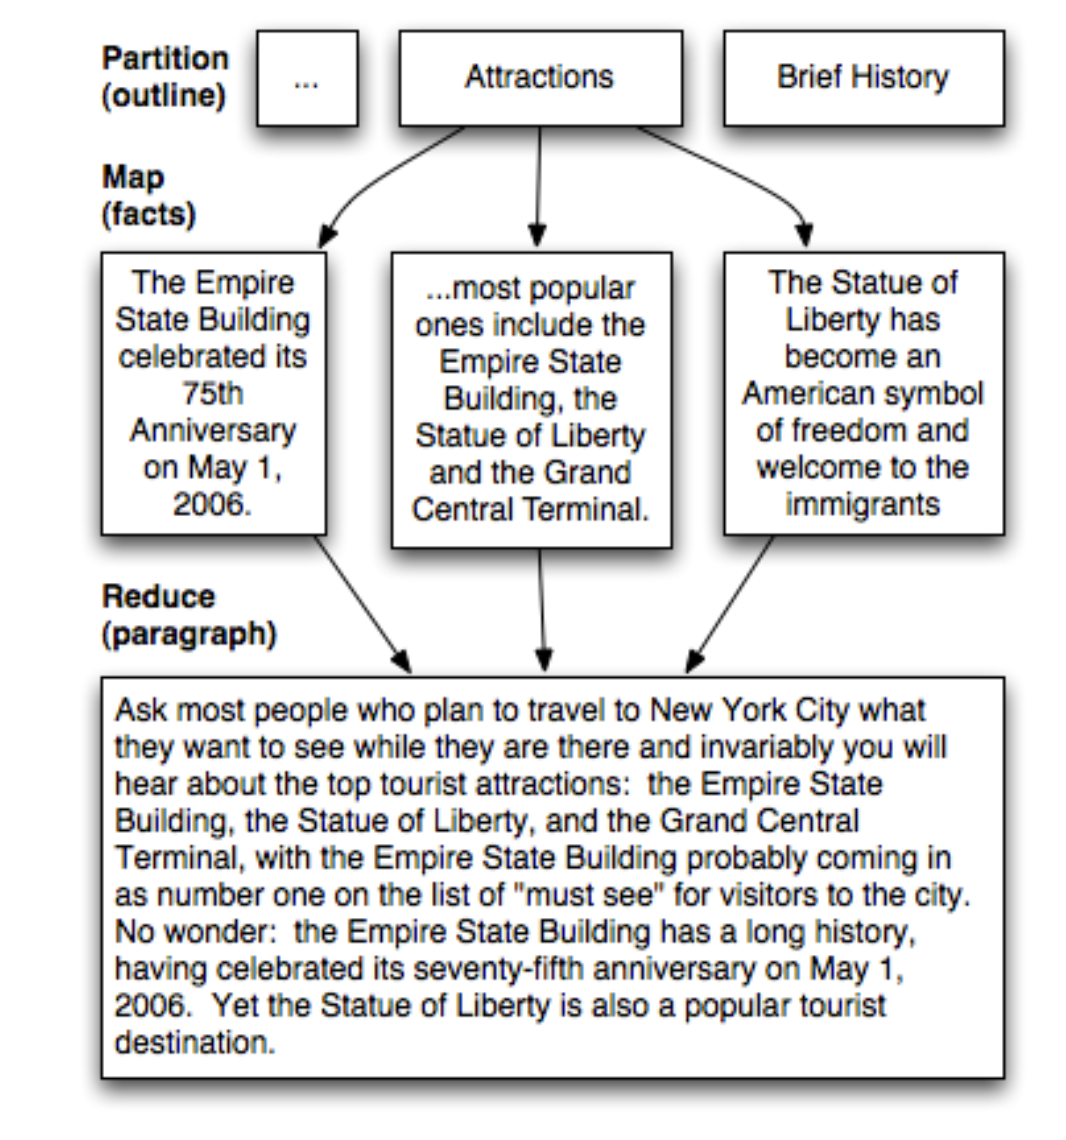
\includegraphics[width=\textwidth]{figures/mapReduce.png}
    \end{figure}
  \end{column}
  
\end{columns}
\end{frame}

\begin{frame}{What does the piecework literature say?}
    something even more insightful, I'm sure!
\end{frame}

\begin{frame}{Comparerereer}
% \framesubtitle{something else}
%   \begin{columns}
%   \begin{column}{0.5\textwidth}
%   % \section*{Piecework}
%      some text here some text here some text here some text here some text here

%   \end{column}

%   \begin{column}{0.5\textwidth}
%   % \section*{CrowdWork}
%      some text here some text here some text here some text here some text here

%   \end{column}
%   \end{columns}
\end{frame}


% \section{Piecework Primer}
% \begin{frame}{Piecework Review
%                                                                                 [\texttt{1 minute}]
% }
% % What is piecework?
% % \begin{figure}

% % \end{figure}
% \end{frame}



\begin{frame}{Contact}

    name: {Ali Alkhatib} \\
    email: \href{mailto:ali.alkhatib@cs.stanford.edu}{ali.alkhatib@cs.stanford.edu} \\
    twitter: \href{https://twitter.com/_alialkhatib}{@\_alialkhatib} \\
\end{frame}


% \bibliographystyle{SIGCHI-Reference-Format}
\printbibliography{}
\end{document} 